\chapter{Einführung}
\section{Aufgabenstellung}
Ziel dieses Praktikums war es eine Software zu konstruieren um \QRCodes in Bildern zu lokalisieren und danach zu extrahieren.
Dabei sollten sich die Teams auf \QRCodes, die dem ISO/IEC Standard 18004 entsprechen, beschränken.
Unter der Annahme, dass sämtliche \QRCodes auf den Eingabebildern planar waren, sollten perspektivische Transformationen oder ähnliche Verzerrungen entfernt werden.
Zusätzlich sollte sich jedes Team darum kümmern ein \emph{Dataset} zur Analyse und späteren Evaluation zu erschaffen.
 
\section{Aufbau des \QRCodes}
Um das spätere Vorgehen der Lokalisierung des \QRCodes nachvollziehen zu können, wollen wir kurz auf den Aufbau des \QRCodes eingehen.
Wie in der Abbildung \ref{fig:struktur-qrcode} zu sehen ist, sind im Code die Informationen zur Version, Format und der Fehlerkorrektur enthalten. 

\begin{figure}[h]
\centering
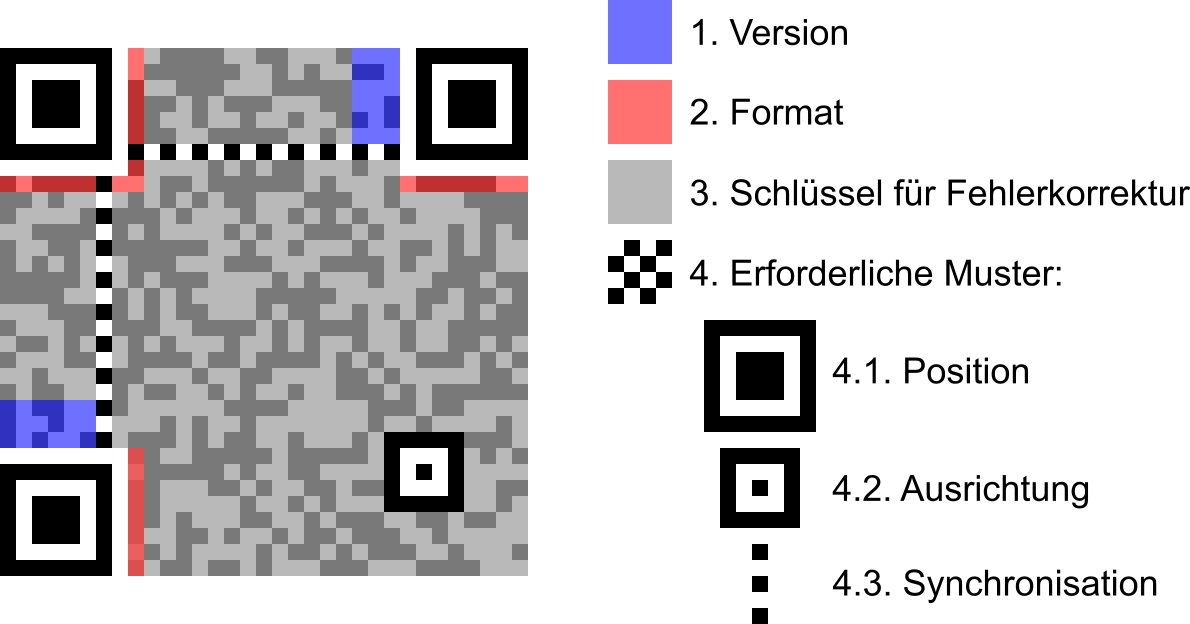
\includegraphics[scale=0.3]{images/QR_Code_Struktur_Beispiel.png}
\label{fig:struktur-qrcode}\caption{\QRCode Strukturbeispiel (siehe Quelle \cite{qrcoderef})}
\end{figure}


Des weiteren ist klar zu erkennen, dass der Code in drei von vier Ecken das Muster 4.1 vorweist. Diese dienen zur Bestimmung der Orientierung. Zusätzlich wird das Muster 4.2 (\emph{Finder Pattern}) verwendet um die Ausrichtung noch prezieser zu bestimmen. Bei größeren \QRCodes werden weitere Ausrichtungsmuster (Muster 4.2) eingefügt. Zwischen den \emph{Finder Patterns} befindet sich ein Streifen mit abwechselnd \glqq schwarz - weißen\grqq\  Punkten (\emph{Modulen}). Das sind die so genannten Synchronisations Muster oder auch \emph{Timming Patterns}.

Die Größe der \QRCodes ist beschränkt durch die Anzahl der \emph{Module}. Die Anzahl der \emph{Module} liegt zwischen $21 \times 21$ und $177 \times 177$. Beispielsweise sei der Code in Abbildung \ref{fig:struktur-qrcode} einer der Größe $21 \times 21$. Dann hätte ein \emph{Finder Pattern} die länge von $7$ \emph{Modules}. Die Anzahl ergibt sich aus der einzigartigen $1:1:3:1:1$ Struktur eines \emph{Finder Patterns}. Diese Fakten werden später ausschlagegebend sein bei der Rasterisierung des \QRCodes.

\section{Die verwendette Bibliothek OpenCV}
\OpenCV\footnote{WWW-Seite von dem Projekt \OpenCV: \url{http://opencv.org/}} ist eine Bibliothek mit Algorithmen spezialisiert auf \glqq Computer Vision\grqq . Sie wurde für die Programmiersprachen C/C++ geschrieben und steht unter BSD Lizenz. Es gibt mehrere Versionen der Bibliothek, die aktuellste ist die 3.2. Unser Programm setzt  die mindestanforderung auf Version 2.4. Außer \OpenCV wurde keine weitere Bibliothek verwendet. 



